\documentclass[letterpaper]{article}
\usepackage[margin=1in]{geometry}
\usepackage[utf8]{inputenc}
\usepackage{textcomp}
\usepackage{amssymb}
\usepackage{natbib}
\usepackage{graphicx}
\usepackage{gensymb}
\usepackage{amsthm, amsmath, mathtools}
\usepackage[dvipsnames]{xcolor}
\usepackage{enumerate}
\usepackage{mdframed}
\usepackage[most]{tcolorbox}
\usepackage{csquotes}
% https://tex.stackexchange.com/questions/13506/how-to-continue-the-framed-text-box-on-multiple-pages

\tcbuselibrary{theorems}

\newcommand{\R}{\mathbb{R}}
\newcommand{\Z}{\mathbb{Z}}
\newcommand{\N}{\mathbb{N}}
\newcommand{\Q}{\mathbb{Q}}
\newcommand{\C}{\mathbb{C}}
\newcommand{\code}[1]{\texttt{#1}}
\newcommand{\mdiamond}{$\diamondsuit$}
\newcommand{\PowerSet}{\mathcal{P}}
\newcommand{\Mod}[1]{\ (\mathrm{mod}\ #1)}
\DeclareMathOperator{\lcm}{lcm}

%\newtheorem*{theorem}{Theorem}
%\newtheorem*{definition}{Definition}
%\newtheorem*{corollary}{Corollary}
%\newtheorem*{lemma}{Lemma}
\newtheorem*{proposition}{Proposition}


\newtcbtheorem[number within=section]{theorem}{Theorem}
{colback=green!5,colframe=green!35!black,fonttitle=\bfseries}{th}

\newtcbtheorem[number within=section]{definition}{Definition}
{colback=blue!5,colframe=blue!35!black,fonttitle=\bfseries}{def}

\newtcbtheorem[number within=section]{corollary}{Corollary}
{colback=yellow!5,colframe=yellow!35!black,fonttitle=\bfseries}{cor}

\newtcbtheorem[number within=section]{lemma}{Lemma}
{colback=red!5,colframe=red!35!black,fonttitle=\bfseries}{lem}

\newtcbtheorem[number within=section]{example}{Example}
{colback=white!5,colframe=white!35!black,fonttitle=\bfseries}{def}

\newtcbtheorem[number within=section]{note}{Important Note}{
        enhanced,
        sharp corners,
        attach boxed title to top left={
            xshift=-1mm,
            yshift=-5mm,
            yshifttext=-1mm
        },
        top=1.5em,
        colback=white,
        colframe=black,
        fonttitle=\bfseries,
        boxed title style={
            sharp corners,
            size=small,
            colback=red!75!black,
            colframe=red!75!black,
        } 
    }{impnote}
\usepackage[utf8]{inputenc}
\usepackage[english]{babel}
\usepackage{fancyhdr}
\usepackage[hidelinks]{hyperref}

\pagestyle{fancy}
\fancyhf{}
\rhead{CSE 101}
\chead{Wednesday, January 12, 2022}
\lhead{Lecture 5}
\rfoot{\thepage}

\setlength{\parindent}{0pt}

\begin{document}

\section{Connectivity in Digraphs}
How do we achieve a clean description of reachability in a directed graph? 
\begin{itemize}
    \item Note that reachability is no longer symmetric. That is, we can reach $w$ from $v$ but not the other way around. 
    \item Can we maybe allow reachability in either direction?
    \item Maybe we can allow the ability to follow edges in either direction? However, this treats a digraph as an undirected graph. 
\end{itemize}

\subsection{Strongly Connected Components}
\begin{definition}{Strongly Connected Components}{}
    In a directed graph $G$, two vertices $v$ and $w$ are in the same \textbf{strongly connected component} if $v$ is reachable from $w$ and $w$ is reachable from $v$.
\end{definition}

\subsection{Equivalence Relation}
Let $v \sim w$ if $v$ is reachable from $w$ and vice versa.
\begin{proposition}
    This is an equivalence relation. Namely:
    \begin{itemize}
        \item $v \sim v$ ($v$ is reachable from itself).
        \item $v \sim w \implies w \sim v$ (relation is symmetric).
        \item $u \sim v \text{ and } v \sim w \implies u \sim w$.
    \end{itemize}
\end{proposition}

\subsection{Relationship to Components}
Essentially, when we have this equivalence relation, we can split a set into components (equivalence classes) so that $v \sim w$ if and only if $v$ and $w$ are in the same component.

\bigskip 

Take any $v$, the set of all $w$ so that $v \sim w$ is the component of $v$. Then, everything connects to everything else in this equivalence class and does not connect (both ways) to anything outside. 

\subsubsection{Example: SCCs}
Consider the following graph:
\begin{center}
    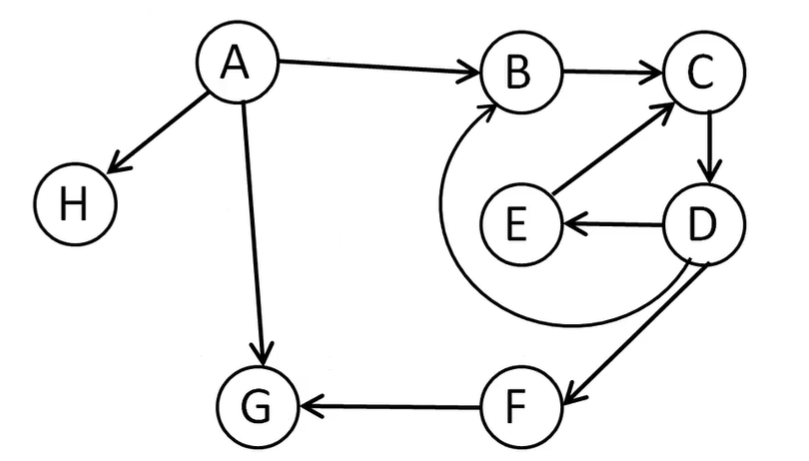
\includegraphics[scale=0.4]{../assets/scc.png}
\end{center}
How many strongly connected components does this graph have? 

\begin{mdframed}[]
    The answer is \textbf{5}. If we use the idea of equivalence classes above, then the equivalence classes are: 
    \begin{itemize}
        \item $B$, $C$, $D$, $E$. 
        \item $A$
        \item $H$
        \item $G$
        \item $F$
    \end{itemize}
    Here, we note that $B$, $C$, $D$, and $E$ are all reachable from each other. However, these vertices and, for example, $A$ are not reachable both ways. 
\end{mdframed}

\subsection{Connectivity}
Do strongly connected components completely describe connectivity in $G$?
\begin{itemize}
    \item \textbf{No}. In directed cases, we can have an edge between strongly connected components. In the undirected case, connected components told you everything that there was to know. However, in the directed case, we can have these two strongly connected components consisting of just a single vertex $v$ and $w$. However, just knowing these components doesn't tell you if there is an edge from $v$ to $w$ or vice versa. There could be an edge that could be extra information that we need to know. 
    \begin{verbatim}
        [v] ---------> [w]
    \end{verbatim}

    \item We need extra information to describe how SCCs connect. 
\end{itemize}

\subsection{Metagraph}
\begin{definition}{Metagraph}{}
    The \textbf{metagraph} of a directed graph $G$ is a graph whose vertices are the strongly connected components of $G$, where there is an edge between $C_1$ and $C_2$ if and only if $G$ has an edge between some vertex of $C_1$ and some vertex of $C_2$. 
\end{definition}
\textbf{Remark:} If you're given the strongly connected components and the metagraph of a graph $G$, then you can you can figure out connectivity within the full graph.

\bigskip

So, the corresponding metagraph of the above graph in the example would be: 
\begin{center}
    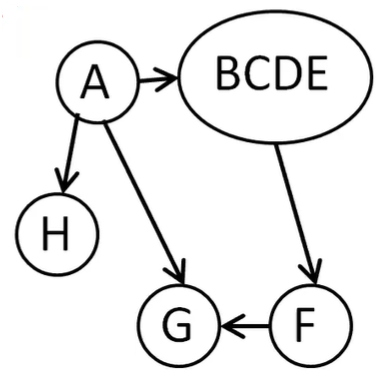
\includegraphics[scale=0.6]{../assets/scc_meta.png}
\end{center}

\subsubsection{Result}
\begin{theorem}{}{}
    The metagraph of any directed graph is a DAG. 
\end{theorem}

% 24:22
\begin{mdframed}[]
    \begin{proof}
        Assume for the sake of contradiction that it is not a DAG. Then, the metagraph has a cycle. Now, let's suppose we have a bunch of strongly connected components; call these SCCs $C_1, C_2, \dots, C_n$. Then, since the metagraph has a cycle, then the strongly connected components form a cycle. That is, we can go from $C_1$ to $C_2$ to $C_n$ back to $C_1$. However, this implies that we have one giant strongly connected component since we can get from one $C_i$ to another $C_j$ ($i \neq j$) and vice versa.     
    \end{proof}
\end{mdframed}


\subsection{Computing SCCs}
Given a directed graph $G$, compute the SCCs of $G$ and its metagraph. 

\subsubsection{Easy Algorithm}
\begin{itemize}
    \item For each $v$, compute vertices reachable from $v$.
    \item Find pairs $v$, $w$ so that $v$ reachable from $w$ and vice versa.
    \item For each $v$, the corresponding $w$'s are in the SCC of $v$.
\end{itemize}
The runtime is $O(|V|(|V| + |E|))$.

\subsubsection{Observation and Better Algorithm}
Suppose that $SCC(v)$ is a sink in the metagraph.
\begin{itemize}
    \item $G$ has no edges from $SCC(v)$ to another $SCC$. 
    \item We can run \code{explore(v)} to find all vertices reachable from $v$. This will contain all vertices in $SCC(v)$. But, it contains no other vertices. 
    \item If $v$ is in the SCC, then \code{explore(v)} finds exactly $v$'s component. 
\end{itemize}
With this observation, we consider the following strategy:
\begin{itemize}
    \item Find $v$ in a sink SCC of $G$. 
    \item Run \code{explore(v)} to find the component $C_1$.
    \item Repeat process on $G \setminus C_1$.
\end{itemize}
The problem is, how do we find $v$ that is in a sink?
\begin{proposition}
    Let $C_1$ and $C_2$ be SCCs of $G$ with an edge from $C_1$ to $C_2$. If we run \code{DFS} on $G$, the largest postorder number of any vertex in $C_1$ will be larger than the largest postorder number in $C_2$. 
\end{proposition}

The reason why we care is because if $v$ is the vertex with the largest postorder number, then: 
\begin{itemize}
    \item There is no edge to $SCC(V)$ from any other SCC. 
    \item SCC is a \underline{source} SCC.
\end{itemize}
However, we wanted a \emph{sink} SCC. So, how do we relate these two?
\begin{itemize}
    \item A sink is like a source, only with edges going in the opposite direction.
\end{itemize}
So, we define a reverse graph like so: 
\begin{definition}{Reverse Graph}{}
    Given a directed graph $G$, the \textbf{reverse graph} of $G$ (denoted $G^R$) is obtained by reversing the directions of all the edges of $G$.
\end{definition}
Some properties of reverse graphs are: 
\begin{itemize}
    \item $G$ and $G^R$ have the same number of vertices and edges. 
    \item $G = (G^R)^R$. 
    \item $G$ and $G^R$ have the same SCCs. 
    \item The sink SCCs of $G$ are the source SCCs of $G^R$. 
    \item The source SCCs of $G$ are the sink SCCs of $G^R$. 
\end{itemize}

The better algorithm we have is: 
\begin{verbatim}
    SCCs(G)
        Run DFS(G^R), record postorder 
        Find v with largest v.post 
        Set all vertices unvisited 
        Run explore(v)
        Let C be the visited vertices 
        Return SCCs(G - C) union {C}
\end{verbatim}

\end{document}